	
	\chapter{Overview on Machine Learning Applied to Satellite Communications}\label{ch:bg}
	
		\par In this chapter, an overview of the SCaN Testbed Cognitive Engine (CE) is provided. In order to understand and motivate decisions that were made in the initial development, general concepts of machine learning will first be discussed. Then, the work accomplished through NASA's SCaN Testbed project prior to this thesis will be described. After this, topics that are relevant to the improvements introduced to the CE by this thesis will be discussed. Finally, the chapter will be summarized.
	\section{A General Overview of Machine Learning}\label{bg:introToML}
	\par With the advent of increasingly more capable and accessible processors, machine learning has become a useful tool in many different fields\cite{MLSurvey_networking} \cite{MLSurvey_medImage} \cite{MLSurvey_general}. This is in part driven by the flexibility and efficiency that machine learning is capable of. There are three major categories of ML algorithms\cite{introToML}: supervised learning, unsupervised learning, and reinforcement learning. Supervised learning takes a set of input values $X$ and a set of target results $Y$ in order to create a mapping $x \to g(x)\to y$. Once the algorithm is trained, this mapping $g(x)$ can be used with new input values $x_{new}$ to predict new target values $y_{new}$. This process is shown in Figure \ref{bg:SupLearnEx}. Unlike supervised learning, unsupervised learning is only given a set of input values $X$. With this set of input values, unsupervised learning attempts to understand the inherent structure within the input values\cite{introToML}. In more general terms, unsupervised learning is attempting to make inferences based on the $X$ given to it. Reinforcement learning is unlike either of the two previously described categories. The primary focus of reinforcement learning is to understand the environment surrounding the learning agent by mapping situations to actions based on maximizing a reward value \cite{rlIntro}. Different supervised learning, where there is an $X$ and $Y$ given to find $g(x)$, reinforcement learning algorithms have $X$ and some knowledge of the reward behavior of the environment $R(x)$, and are trying to choose $X$ in order to get a large $Y$ while simultaneously expanding its knowledge of $R(x)$.  
	
	\begin{figure}[ht]
		\begin{center}
		\begin{subfigure}{\linewidth}
		\centering
		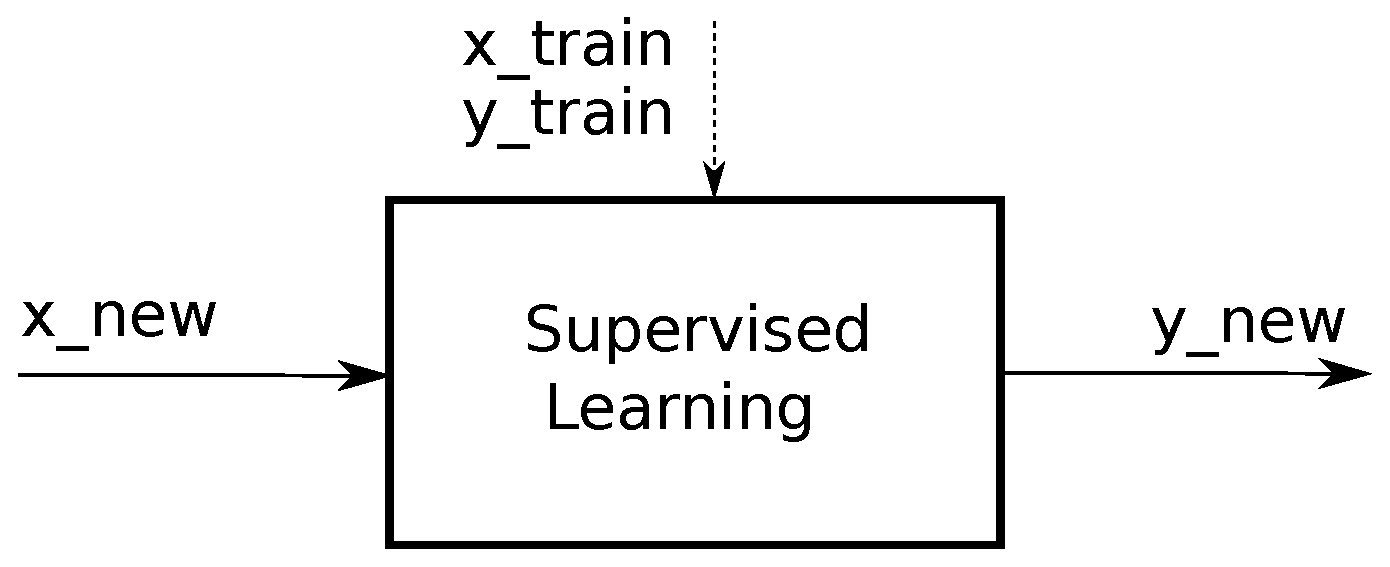
\includegraphics[scale=0.4]{figures/supervisedLearningBlock.eps}
		\caption{Supervised Learning Block Diagram.}
		\end{subfigure}
		\end{center}
		\begin{center}
		\begin{subfigure}{\linewidth}		
		\centering
		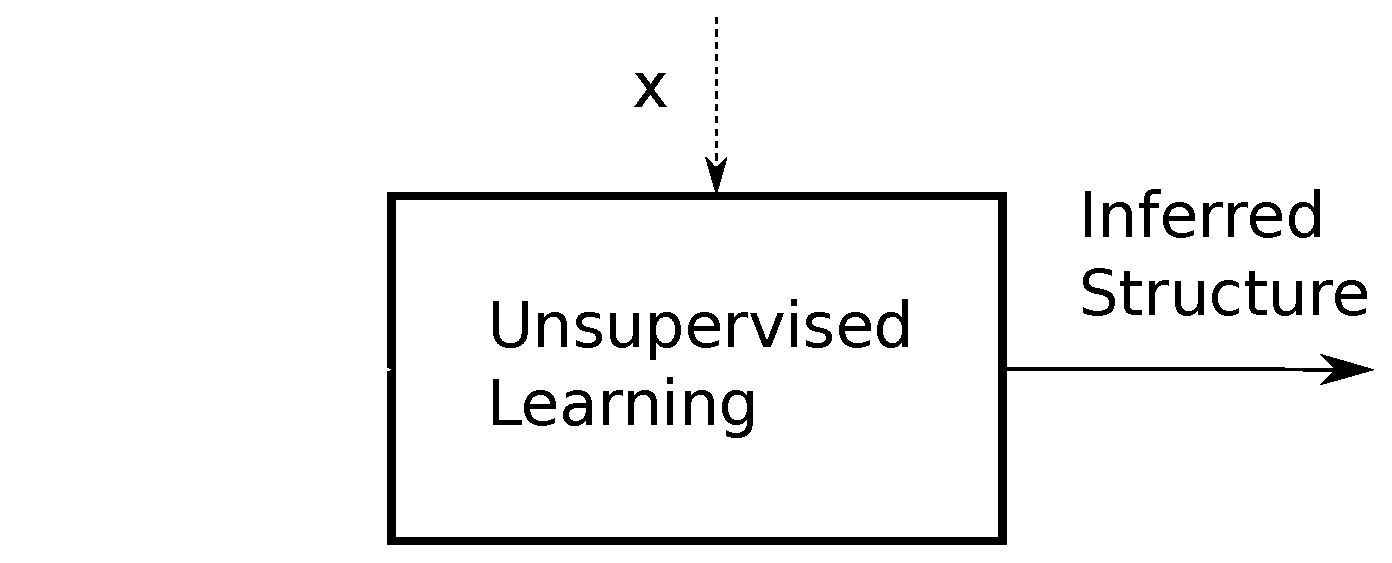
\includegraphics[scale=0.4]{figures/unsupervisedLearningBlock.eps}
		\caption{Unsupervised Learning Block Diagram.}
		\end{subfigure}
		\end{center}
		\begin{center}
		\begin{subfigure}{\linewidth}
			\centering
			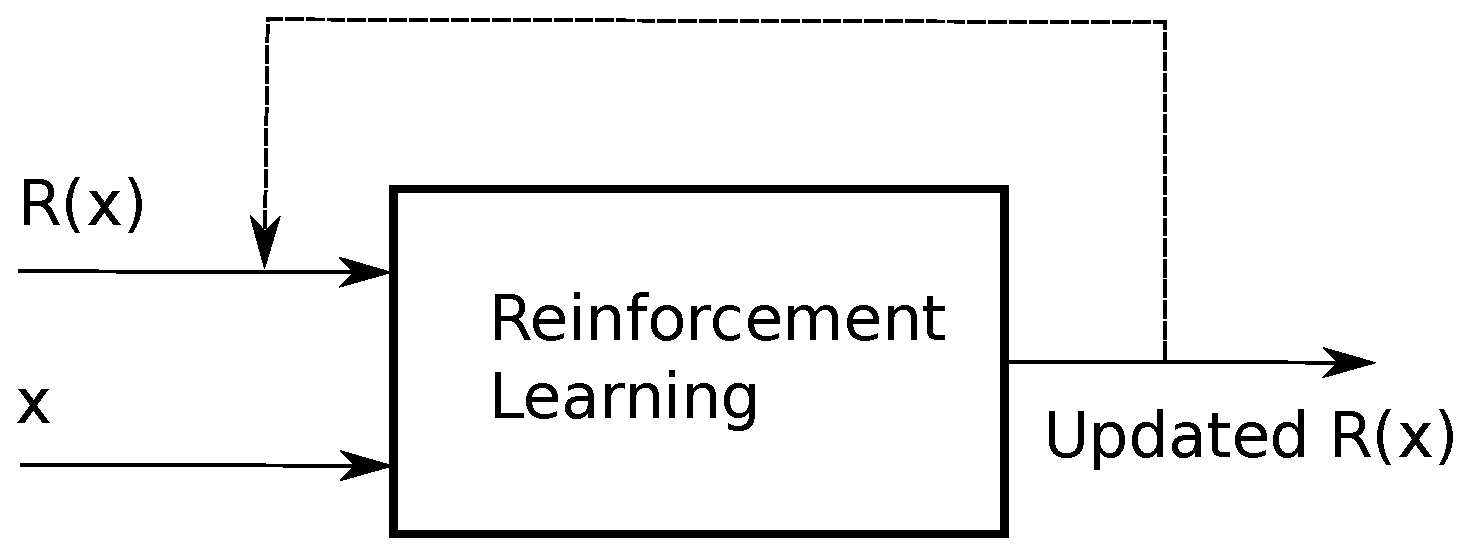
\includegraphics[scale=0.4]{figures/reinforcementLearningBlock.eps}
			\caption{Reinforcement Learning Block Diagram.}
		\end{subfigure}
		\end{center}
		\caption{Flow diagrams of the three main categories of Machine Learning.}\label{bg:SupLearnEx}
	\end{figure}

	\begin{figure}[ht]
		\centering
		\caption{Basic overview of different machine learning techniques.}
		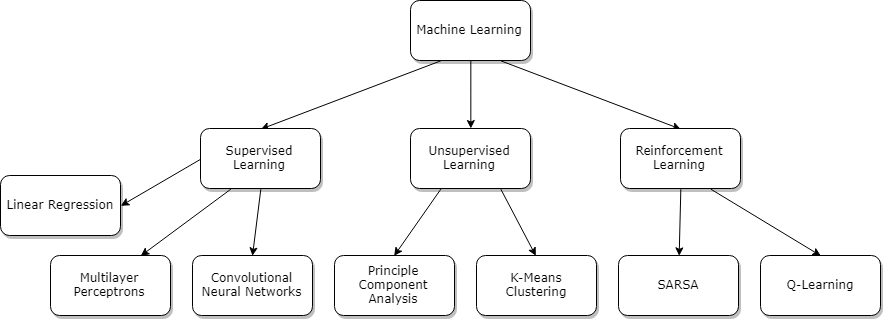
\includegraphics[scale=0.5]{figures/MLdiagram.png}
	\end{figure}
	%\par \textbf{\textit{Decide if I want to include actions as part of RL diagram}}
	
	\par Within the CE, concepts from Supervised Learning and Reinforcement Learning are used. As such, the rest of this section will focus on those two categories in more detail.% \cite{placeholderCitation}. 
	\subsection{Supervised Learning}
	\par As stated before, supervised learning refers to the problem of modeling some sort of relation between two sets of data: an input dataset and a target dataset. This problem is further subdivided into two different types of problems: regression and classification. Regression refers to the modeling of a continuous target. One common example is the modeling of the cost of a house based on its square footage. $x$ in this case would be the square footage of the house, and $y$ would be the cost of the house. Regression refers to the fact that the cost of a house can have any value within a range. The other type of problem is classification, which models a discrete target. This is the act of assigning input values to one of a number of different classes. A simple to understand example is determining if someone is likely to renew a magazine based on their age. In this case $x$ is the age of the subscriber, and $y$ is whether or not the subscriber will renew their subscription. This is classification because there are two discrete possibilities for $y$, that the subscriber will renew their subscription and that the subscriber will not renew their subscription.  
	\par In order to train a model for either problem class, a set of training data similar to the expected input is required, $X_{train}$. In addition to the input set, the corresponding target values are needed as well, $Y_{train}$. With this information, the chosen algorithm is trained to understand the nonlinear mapping from input to target. Once the algorithm is trained, it will take inputs $X$ and predict the resulting value of $Y$. There are a wide variety of algorithms that are applied to supervised learning. Some relevant algorithms include Linear Regression, Classification and Regression Trees (CART), Multilayer Perceptrons/Feed Forward Neural Networks (MLP/FFNN), and Convolutional Neural Networks (CNN). Each of these algorithms has its own training method. A focused description of the training algorithms for CART and MLP will be provided. CART was chosen because of the relative ease of explanation and the fact that it is often used as a baseline of performance to compare to. MLP was chosen because it is the method used in CE.
	\par The CART is one of the most basic supervised learning techniques still in use today. For each input vector $\vec{x} \in X$, a series of decisions are made based on the values of $\vec{x}$. At each decision, the possible state of the tree is split in two, depending on which value $\vec{x}$ takes. Once there are no more splits, the tree comes to either a class (for classification) or a value (for regression) for $\vec{x}$. This is more thoroughly described in Algorithm \ref{code:bg_cart}.
	\begin{algorithm}[ht]
		\caption{CART Pseudoalgorithm [Note, these variables are not in the text] }
		\label{code:bg_cart}
		\begin{algorithmic}[1]
			\Procedure{CART}{}
			\While{$leafNotReached$}
			\State $x = x_{eval} \in X$
			\If {$x > \textit{branchValue}$} Branch right.
			\Else \ Branch left.
			\EndIf
			\EndWhile
			\State \Return $leafValue$ or $leafClass$
			\EndProcedure
		\end{algorithmic}
	\end{algorithm}

	\par One benefit of this algorithm is that it is fairly intuitive, behaving in a way that is similar to how a human might make a decision. It is also fairly simple, not making any underlying assumptions about the underlying data or requiring any parameters. This allows CART to be applied in a fairly straighforward manner to a wide variety of problems. One downside of CART is that it's simplicity makes the method prone to overfitting. Given $n$ inputs, a tree that splits $n-1$ ways would be capable of 100\% accuracy on the training dataset. However, it would likely underperform on any other data, with stochastic processes or non-generalizable patterns perturbing the data beyond the behavior the tree learned. As a result of this, algorithms must be careful to train only until the tree meets the expected specifications in regards to accuracy and other performance metrics. In addition, pruning techniques to remove non-generalizable branches are employed. When this issue is taken into account, CARTs act as a good baseline algorithm. This has resulted in them being used in many ensemble-based methods, which use multiple copies of an algorithm to produce results. Ensemble-based methods will be discussed in further detail in Section \ref{bg:advanced_ensemble}.
	
	\par While CART is a simple and useful method, the recent resurgence of Machine Learning as a useful field has been driven by extensions of the multilayer perceptron (MLP)\cite{deepLearningSurvey}, also known as the feedforward neural network (FFNN). An MLP is composed of layers. Each layer is itself composed of nodes, each of which holds a value. The inherent meaning of a node value depends on what type of layer the node belongs to. There are three different types of layers: input layers, hidden layers, and output layers. For each MLP there is one input layer, which is composed of inputs $x_i$. Each hidden layer node is a linear combination of all the nodes from the layer before it. How much each node from the previous layer impacts the current node is defined by a set of weights and biases. After this linear combination, the node applies a nonlinear transform, often called the activation function. Frequently, this transform is used as a squashing function to limit the outputs to a certain range\cite{sigmoidReason}. Some examples of this are the tanh() function, which limits the range to (-1,1), and the logistic function, which limits the range to (0,1). Non-linearities are introduced to allow the MLP to represent more complex relationships. Without the activation function, adding additional layers would not result in any increase in representational ability. The output layer takes the values from the last hidden layer and, after one more linear combination, outputs the MLP's prediction of the target value. 
	 % Maybe put a subheader here because it is sort of a break.
	\par In order to train an effective model, there needs to be a way to evaluate how effective the model is at any given moment. For an MLP, this is accomplished by using a cost function $J$, which is used to evaluate how well the model is performing compared to the ground truth. In the context of a classification problem, a commonly used cost function is cross-entropy, also known as log loss. Cross-entropy, a concept taken from information theory, represents the average number of bits needed to identify if a sample was taken from probability distribution $p$ or probability distribution $q$. By choosing $p=y_{truth}$ and $q=y_{pred}$, cross-entropy can be used as a distance metric. A commonly used cross-entropy based cost function is described in Equation (\ref{eq:bg_crossentropy}) \cite{lossFcns}, where $y$ is a binary indicator, with 0 and 1 representing the two different classes that the model is choosing between. By using this formulation, the only factor to loss is the class predicted. 
	\begin{align}
		J_{crossEntropy} &= \frac{\sum_N (y_{truth}log(y_{pred}) + (1-y_{truth})log(1-y_{pred})) }{N} \label{eq:bg_crossentropy} 
	\end{align}
	\par This error function is based on a binary classification problem, but can be easily extended to a multi-class problem by using a separate binary classification for each class, and sum the cross-entropic error for each class to get the total cross-entropic error.  
	\par In the context of a regression problem, a commonly used cost function is mean squared error (MSE). The definition of MSE is given in Equation (\ref{eq:bg_mse}) \cite{lossFcns}. As the name implies, it represents the mean of the squared error between the $y_{pred}$ and $y_{truth}$. Unlike Equation (\ref{eq:bg_crossentropy}), $y$ here represents a continuous value, so the distance of the prediction to the truth value impacts the metric. 
	\begin{align}
		J_{MSE} &= \frac{\sum_N (y_{pred}-y_{truth})^2}{N} \label{eq:bg_mse}
	\end{align}
	\par By using these cost functions, a clearer picture about the effectiveness of a model is created. With training reframed as an optimization problem, the simplest solution is to use gradient descent. Upon taking the gradient of the cost function, the resulting value willbe negative for downward slopes and positive for upward slopes. By updating the weights in the opposite direction of the gradient, the resulting loss value from the updated network will move towards a minimum. This is represented in Equation (\ref{eq:bg_gradDescent}) \cite{backpropIntro}, where $h$ represents the value to change the weights $W$, and $J$ is the Jacobian (the matrix of all first-order partial derivatives of a vector) of the objective function. This method converges well with simpler objective functions, but has the potential to converge slowly, depending on the $\alpha$ parameter and the Jacobian.
	\begin{align}
		h_{gd} &= \alpha J^T W(y_{truth}-y_{pred}) \label{eq:bg_gradDescent}
	\end{align}
	\par Another solution is called the Gauss-Newton method \cite{gauss_newton_alg}, which is applicable to a sum-of-squares objective function, like $J_{MSE}$. It assumes that the objective function is approximately quadratic near the solution, then uses a first-order Taylor series expansion to approximate the Hessian of the objective function to be $J^TWJ$. This then allows for the weight update procedure to follow Equation (\ref{eq:bg_gaussNewton}). This converges much faster than gradient descent for moderately-sized problems, but is only applicable to a stricter set of objective functions, as it depends on the function being twice differentiable. It also doesn't provide as much of a speedup when the first derivative of the objective function has repeated roots. 
	\begin{align}
		h_{gn} &= (J^TW(y_{truth}-y_{pred}))(J^T WJ)^{-1} \label{eq:bg_gaussNewton}
	\end{align}
	\par The solution that is frequently used (and is the MATLAB default in training a neural network) is the Levenberg-Marquardt (LM) method\cite{lm_alg}. This is effectively a combination of the two prior optimization methods. It is described in Equation \ref{eq:bg_lm}. 
	\begin{align}
		h_{lm} &= (J^TW(y_{truth}-y_{pred}))(J^T WJ + \lambda \cdot diag(J^T WJ))^{-1} \label{eq:bg_lm}
	\end{align}
	\par The variable $\lambda$ represents the parameter that controls how similar the update is to Gradient Descent, and how similar the update is to Gauss-Newton. A large $\lambda$ makes LM more similar to Gradient Descent, and a small $\lambda$ makes LM more similar to Gauss-Newton. The variable $\lambda$ is usually initialized to be large, to enable the first updates to be small. If an update increases the objective function, than $\lambda$ is increased, moving closer to Gradient Descent. Otherwise, $\lambda$ decreases, moving closer to Gauss-Newton. This is reasonable because as the weights approach the optimal solution, it is more reasonable to assume that the cost function is quadratic.
	\par For an algorithm like linear regression, one of these update methods by itself is enough as an update procedure. However, MLPs require a modification of this process. This is due to the multiple layers involved, which introduce additional complexity with the interconnections between layers. The process of updating MLPs is called Backpropagation. Gradient Descent Backpropagation will be described in Algorithm \ref{alg:bg_gdBackprop}, as it is the simplest to understand. Backpropagation as applied to Levenberg-Marquardt can be found in \cite{placeholderCitation}.
	%label{code:bg_backprop}
	\begin{algorithm}
		\caption{Pseudocode for Backpropagation}
		\label{alg:bg_gdBackprop}
		\begin{algorithmic}[1]
			\State Given: training set $X$.
			\Procedure{Backpropagation}{}
			\State Set input activation $a^1=\sigma(X)$
			\For{$l=2$:$L$}
			\State $z^l = w^l a^{l-1} +b^l$
			\State $a^l = \sigma(z^l)$ 
			\EndFor
			\State $\delta^L = \nabla_a C \odot \sigma '(z^L)$
			\For{$l=L-1$:$2$}
			\State $\delta^l = (w^{l+1}\delta^{l+1}) \odot \sigma '(z^l)$
			\EndFor
			\State Output 1: $\frac{\delta C}{\delta w^{l}_{jk}} = a^{l-1}_{k}\delta^{l}_{j}$
			\State Output 2: $\frac{\delta C}{\delta b^{l}_{j}} = \delta^{l}_{j}$
			\EndProcedure
		\end{algorithmic}
	\end{algorithm}
	\par The symbol $\odot$ is the Hadamard Product, which is an element-wise product of two vectors with the same length. $L$ is the number of layers in the MLP. $z^l$ is the weight and bias values at layer $l$, and $a^l$ is $z^l$ passed through the activation function $\sigma(z)$. $\delta^l$ is the error at layer $l$.
	\par The backpropegation algorithm used in MLPs can be broken into 4 steps: forward propegation, backpropegation at the last layer, backpropegation at the hiden layers, and updating of the weights. 
	Forward propegation is simply applying the training inputs to the network as normal (represented by steps 2-6). Then, the backpropegation error at the output is calculated (step 7). Then, the error is carried back through the network in the same way that the MLP is applied, except backwards. Once this is done, the partial derivatives of each node will be calculated, and can be used in a gradient descent manner. 
	\begin{figure}
		\centering
		\caption{A flow diagram describing gradient descent.\textit{\textbf{[make a flow diagram ]}}}\label{bg:flowBackProp}
		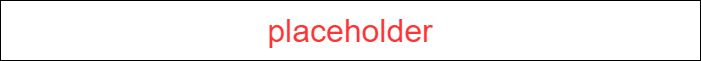
\includegraphics[scale=0.5]{figures/Placeholder.png}
	\end{figure}
	\par In recent times, improved versions of backpropegation have been proposed and utilized, such as RMSprop and Adam. Both of these improvements are extensions of standard gradient descent backpropegation. Standard backpropegation utilizes one learning rate for all weight updates. This rate doesn't change during training. RMSprop, also known as Root Mean Square Propagation, maintains per-parameter learning rates that get adjusted by a moving average of the recent gradient values for the individual weight \cite{RMSPropPaper}. Adam takes this a step further and adapts the parameter learning rates based on the gradient's variance, in addition to the gradient's mean that RMSProp uses. Doing so results in quicker convergence than standard backpropegation. Details can be found in \cite{AdamPaper}. In modern times, Adam has been frequently recommended as the default optimization method in training neural networks\cite{CNNKarpathyClass}. Both RMSProp and Adam are still based on first-order methods, unlike Gauss-Newton and Levenberg Marquardt, which is likely one of the reasons why the new algorithms have surpassed the old ones in usage. Nonetheless, the same concern in online usage remains. This thesis will stick to LM, as the project it is building on top of is based off of LM.
	\par http://cs231n.github.io/ karpathy CNN class
	\par https://page.mi.fu-berlin.de/rojas/neural/chapter/K7.pdf Link to chapter that discusses backprop
	\subsection{Reinforcement Learning}

	\begin{figure}
		\centering
		\caption{An overview of reinforcement learning.\textit{\textbf{[Get figure from paulo's RL diagram]}}}\label{bg:flowRL}
		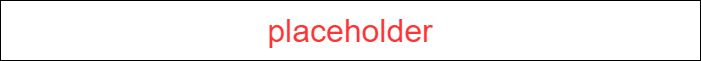
\includegraphics[scale=0.5]{figures/Placeholder.png}
	\end{figure}

	\par While both supervised and unsupervised learning are built on the premise of identifying some form of structure from a given set of data, the goal of Reinforcement Learning (RL) is fundamentally different. The core premise of RL is of an agent trying to learn an environment. In passive RL, there agent has no influence on the environment, and can just observe some reward based on the location it is at. In active RL the agent is able to take actions, and so the reward is based on the location and the action that was taken. With this reward value, the agent can update its understanding of the environment, in a form called the state-transition model. How it does this depends on the RL algorithm being used. Active RL is more relevant to this thesis
	\par While there are multiple different ways to pose an RL problem, the one that is most applicable to the problem at hand is the Multi-armed bandit. In this model, an action set has multiple reward functions, used as metrics for how well a task was executed. 
	The agent is the "bandit", trying to get the "best" reward overall over the multiple reward functions. How best is defined is difficult, as the interaction between reward functions is not straightforward, and the impact of each reward function may vary. 
	 Another potential model is that of a state-transition problem, modeled as a Markov decision process. Rephrased in a RL context, the target problem is changing radio parameters so that optimal performance is achieved in context of the current environmental conditions. There are a wide range of conditions that affect the state-transition model, including the communications channel. This channel is affected by the dynamic geometry of the line-of-sight between the transmitter and receiver, as well as atmospheric and space weather. These complex and changing conditions make finding the state-transition model and action-state mapping analytically an intractable pursuit. 
	\par This difficulty is what makes RL a good fit for tackling the problem. RL makes few assumptions about the behavior of the process being studied, other than the fact that it can be reasonably modelled by a state-transition model. In addition, RL is designed to be constantly used and updated, instead of waiting for the optimal solution to be calculated before running. With these two properties, the primary concern shifts from intractability to ensuring the agent interacts with the environment in an efficient way to find the best possible policy. The best way to form a policy would be to evaluate the action-value function $Q(s,a)$ at each possible state and action. However, this becomes intractable quickly. Instead, the agent periodically explores policies, with either on-policy or off-policy approaches. On-policy approaches affect the policy that the agent uses to make decisions, while off-policy approaches affect a separate policy from the one that the agent uses to make decisions. Since the target platform is a cognitive engine that actively adapts to the environment conditions, the focus will be on-policy approaches. 
	\par The model-free method that is relevant to this thesis is Temporal-Difference (TD). This method updates $Q(s,a)$ using the past experiences at each time step. This makes it useful for time-sensitive applications. When used on-policy, it is called State-Action-Reward-State-Action (SARSA). The pseudoalgorithm for SARSA is provided in Algorithm \ref{code:bg_SARSA}.
	
	\begin{algorithm}[ht]
	\caption{SARSA Pseudoalgorithm}
	\label{code:bg_SARSA}
	\begin{algorithmic}[1]
		\Procedure{SARSA}{}
		\State Initialize $Q(s,a)$ for all states $s$ and actions $a \epsilon \mathcal{A}(s)$ arbitrarily. Set $Q(terminal\ state)=0$.
		\While{Learning}
		\State Initialize $s$
		\State Choose $a$ from $s$ using policy derived by $Q$.
		
		\While{not terminal state}
		\State Take action $a$, observe reward $r$ and next state $s'$.
		\State Choose $a'$ from $s'$ using policy derived from $Q$.
		\State Update Q: $Q(s,a) \gets Q(s,a) + \alpha[r + \gamma Q(s',a')-Q(s,a)]$.
		\State Update $s \gets s'$,$a \gets a'$.
		\EndWhile
		\EndWhile
		\State \Return Updated Q table.
		\EndProcedure
	\end{algorithmic}
\end{algorithm}

		\par $\alpha$ is the learning rate of the algorithm, r is the reward, $\gamma$ is the discount factor for future rewards. In our context, there is no terminal state. The algorithm instead ends when there is no longer a connection between the SCaN testbed and the ground station. Described briefly in words, the SARSA algorithm is as follows. Before running, initialize the Q function for all possible states and actions. Then, initialize the current state, and choose a based on a given policy. Take the action $a$, and observe reward $r$ and state $s'$. Using the same policy based on Q, choose the next action $a'$ given $s'$. From this, update $Q(s,a)$. The value within the brackets is known as TD error, and is the difference between the predicted value of $Q(s_k,a_k)$ and the better prediction of $r + Q(s_{k+1},a_{k+1})$. Then, repeat the process of taking actions and observing rewards. 
	\par In the context of cognitive radio, only the immediate reward (i.e.$\gamma = 0$) is relevant \cite{AIAA_Paper}. In addition, any action can be taken from any state without the need for planning. This results in a modified Q function:
	\begin{align}
		Q_{k+1}(s_k,a_k) &= Q_k(s_k,a_k) + \alpha[r - Q(s_k,a_k)]. \label{eq:bg_sarsa2}
	\end{align}
	\par Based on $Q(s_k,a_k)$, a knowledge base called a Q-table is built up. In this table, previous Q-values are mapped to the state-action pairs that resulted in the Q-values. In SARSA, the value of $Q(s_k,a_k)$ is updated when the action is taken. Beyond $Q(s,a)$, a reward function $r = g(s,a)$ and an exploration policy $a = h(s)$ need to be defined before a practical model is complete. In the context of the CE, a multitude of functions are relevant to the overall performance of the system. These performance functions may or may not have conflicting responses. The reward function mapping environmental information to performance is a combination of values from these performance functions. The overall result is then represented as a percentage of the maximum possible performance value. 
	
	\par One of the most important tradeoffs for RL is deciding how much time should be spent exploring the environment versus how much time should be spent exploiting the knowledge already gathered. This is frequently called the Explore-Exploit tradeoff \cite{placeholderCitation}. In the context of SARSA, exploring would represent choosing an unvisited action while exploiting would be choosing an action that has the highest Q value. The exploration policy is responsible for making this decision. This tradeoff is important because exploring too much would create a detailed understanding of the environment but would not actually use the information, while exploiting too much could be using subpar information as the environment is only minimally explored. The preventing of either of these cases becomes an important issue. 
	\par There are many different approaches to tackling the explore-exploit tradeoff. The simplest one is to use an $\epsilon$-greedy policy \cite{placeholderCitation}. In this method, an  random numbe r$n$ is drawn form $\mathcal{U}(0,1)$. This is compared to $\epsilon \in (0,1)$. If $n<\epsilon$, a random action is chosen. Otherwise, a greedy action based on the Q-table is chosen\cite{placeholderCitation}. $\epsilon$ can be set as a function decreasing over time. This results in more random actions being chosen at the beginning of the running the algorithm and more exploitation of the explored environment as time goes on. Other exploration policies include value-difference based exploration (VBDE) \cite{placeholderCitation}, which changes $\epsilon$ based on TD error, as well as Boltzmann exploration and probability matching \cite{placeholderCitation}. In this work, a time-varying $\epsilon$-greedy policy is used. 
	\par \textit{\textbf{[discuss where NNs slot in]}}
	\section{Previous work on NASA SCaN Testbed}
	\par This section first describes the problem that is trying to be solved by the NASA John H. Glenn Research Center (GRC) Space Communications and Navigation (SCaN) Testbed project \cite{placeholderCitation}. With this foundation, the architecture of the cognitive engine (CE) that was developed will be described as well. Finally, the primary goals of the extension that this thesis is focused on will be described.
	\subsection{Problem statement}
	\par The Cognitive Engine project, and by extension this thesis, is built on top of the SCaN Testbed, an experimental communication system developed by NASA to research implementation solutions for issues related to SDR-based communications to and from space \cite{placeholderCitation_pauloTim}. The platform consists of multiple SDRs that are configured to operate at S-band and Ka-band, both in direct communications to ground stations on Earth and in communication with NASA's satellite relay infrastructure named Tracking and Data Relay Satellite System (TDRSS \cite{placeholderCitation}). For this thesis, communication with ground stations is the central focus. This platform is used to research real-world satellite dynamics between spacecraft and relay satellites or ground stations. Some of the dynamics studied include time-varying Doppler changes, differences in thermal conditions, interference, range variation, ionospheric effects, and other impairments to propagation.
	\par The SDRs chosen for the SCaN testbed are flight-grade systems, fully compliant with NASA's Space Telecommunications Radio System (STRS)\cite{placeholderCitation} SDR architecture. This architecture provides abstraction interfaces between the radio software and proprietary hardware, allowing for third-party software waveforms and applications to interact with and run on the radio. 
	%In the context of communications systems, waveforms refer to the specific PHY standards used when transmitting a message, including the configurable parameters that they specify are allowed. 
	STRS also provides a library of waveforms available that provide various modulation, coding, framing, and data rate options. 
	\par On top of this platform, solutions such as adaptive communications using cognitive decision making can be researched, which will help solve communication issues on Earth as well as allow for the development of space communication systems that will enable space exploration in the near future \cite{paulo_cite_131}. SDRs are important in this development, as their flexibility and reconfigurability provides a strong tool that enables a wide variety of tests. However, SDRs tend to be more complex than traditional fixed-configuration radios. Cognitive radio (CR) systems help reduce the complexity and risk in using these systems. The work that this thesis is extending plays a part in this effort, providing CR algorithm research for SDR systems in space.    
	\par Three areas have emerged as candidate application areas for CR: node-to-node communications, system-wide intelligence, and intelligent internetworking. The first application focuses on radio-to-radio links between mission spacecraft and a ground terminal \cite{placeholderCitation}. Cognitive decisions may improve throughput across the communication link by adjusting waveform settings to maximize user data and symbol rate, while using more conservative settings during parts of the pass with poor channel conditions. The second application is system-wide intelligence, where the CR systems make operational decisions normally performed by operators \cite{placeholderCitation}. For instance, CR systems could be applied to scheduling, asset utilization, optimum link configuration and access times, fault monitoring, and failure prediction, among others. In this application, a CR system could reduce operation oversight and reduce operational complexity, by choosing among the large search space of configurations. The final application of CR systems applies to the network level \cite{placeholderCitation}. With control and data functions of the communications network, CR systems could optimize data throughput using QoS metrics such as bit error rate. Learning network behaviors could enable the CR to provide throughput and reliability benefits.
	\par  For this thesis and the work preceding it, the first application was considered to be the main priority without loss of generality. Regardless of the application, the need for verification and ground-testing of all operational conditions before launch is apparent, since doing so minimizes the risk of malfunction on-orbit. Once this verification is complete, tests (including the one in this thesis) can be conducted in order to more properly study the impact of CR systems on communications.
	\par The project this thesis is extending, titled "Intelligent MAC protocol for SDR-based satellite communications", involved the NASA Glenn Research Center (GRC) such that cognitive engine algorithms for future space-based communications systems can be developed. This effort included the opportunity to perform on-orbit tests with the SCaN Testbed SDRs. This effort's R\&D team is composed of members from WPI and the Pennsylvania State University, in collaboration with the SCaN team at NASA GRC. The project commenced in November 2014, and the initial tests were completed in May 2017. This extension is scheduled to be completed by December 2018.
	\par During the course of this project, the team designed and developed a proof-of-concept of an intelligent MAC protocol to maximize data link performance and improve robustness of space communications systems. This uses SDRs for low margin data links operating on dynamically changing channels. The protocol's core is composed of a Cognitive Engine (CE) that balances multiple different objective issues during radio-resource allocation. Radio parameters may be adapted to mitigate channel impairments or when meeting new performance requests. Key capabilities for cognition are prediction and learning techniques assisted by third-party databases when they are available.  
	\par This CE project aligned specifically with NASA's Communication and Navigation Systems Roadmap Technology Area 5 \cite{placeholderCitation}, which focuses on the concept of a cognitive radio in space that senses the environment, autonomously determines when there is a problem, attempts to fix it, and learns about the environment as they operate. It also acts as a step towards reducing the limits that communication techniques impose on future missions and their critical phases. The CE algorithm, as well as expreiment results, will be used to assess the performance of the adaptive MAC protocol performance for on-orbit SDRs, and will help in the design of future MAC protocols and mitigation techniques that utilize intelligent radio parameter reconfiguration. 
	\par There are four different communication channels between the fixed ground stations at GRC/White Sands, the moving ScaN Testbed SDR on board the ISS, and the TDRSS satellite at a GEO orbit, as illustrated by Figure \ref{fig:exampleCommChannels}. Radio parameter reconfiguration might be done during periods of signal fading, especially those happening during low elevation angles of the SCaN Testbed antenna, while tracking the TDRSS satellite, or low elevation angles from a GRC ground station antenna, while tracking the ScaN Testbed. The project focuses on the direct communication between GRC and the SCaN Testbed.
	\begin{figure}
		\centering
		\caption{Four potential communication channels.}\label{fig:exampleCommChannels}
		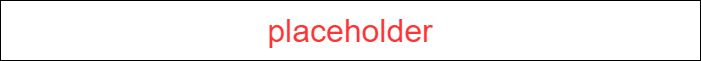
\includegraphics[scale=0.5]{figures/Placeholder.png}
	\end{figure}
	\begin{figure}
		\centering
		\caption{A flow diagram describing the CE's flight-test setup.}
		\label{fig:CE_outline}
		
\includegraphics[scale=0.5]{figures/system_block_diagram.eps}
	\end{figure}
	
	\par A high level overview of the proposed CE is shown in Figure \ref{fig:CE_outline}. The platform gathers telemetry data reported from the transmitter or measured at the receiver. A predictor employs past information to predict which radio parameter values will achieve good performance. Learning techniques are used for prediction in order to control storage memory growth. Decision logic based on the predictions will choose what adaptations will need to occur. The CE learns the environment behavior by building a model that maps observed telemetry data to radio parameter sets. A more detailed representation of he CE is shown in Figure \ref{make this figure too}, and will be discussed in more detail in Section \ref{ch:methods}.
	\begin{figure}
		\centering
		\caption{An overview of the CE.\textit{\textbf{[make MAKETHISFIGURE, eg the CE diagram figure]}}}
		\label{bg:CEFigure}
		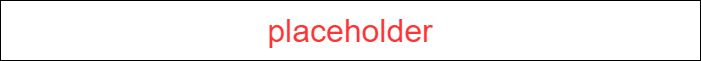
\includegraphics[scale=0.5]{figures/Placeholder.png}
	\end{figure}

	\par In this thesis, the goals were twofold: To explicitly deal with the catastrophic forgetting that occurs in MLPs, and to investigate the potential utility of GANs. In the following section, both of these subjects will be discussed in more detail.
	
	\section{Advanced Topics in Machine Learning}
	\par \textbf{\textit{[Intro paragraph needed]}}
	\subsection{Online Learning and Catastrophic Forgetting}\label{bg:onlineLearning}
	\par In supervised learning, there are two different learning paradigms: Online learning and offline learning. Offline algorithms assume that there is one set of inputs and outputs to train on, and that once training is complete there will be no updates to the algorithm. The training methods described in Section \ref{bg:introToML} are all considered to be offline methods. This is contrasted with online algorithms, which update as new data is received. The choice between an offline algorithm and an online algorithm is dependent on the problem that is selected. With a stationary dataset, a single training period can be sufficient. However, if the dataset is nonstationary, there is a reason for multiple training periods capturing the shifting of the data, also known as concept drift \cite{placeholderCitation}. Since effective space communications systems are dependent on many nonstationary variables, online methods are more suited for this project.
	\par The most basic category of online methods consists of generalizations of offline methods. In this category, a window of incoming data is collected. Once this window is full, the collected data is used to train using an offline method. Then, some number of datapoints are dropped and the window is filled again. This moving window process is the most straightforward extrapolation of offline algorithms. In the baseline CE, this method is applied to LM \cite{placeholderCitation}. The moving-window approach has one major problem that it introduces. The LM algorithm updates the weights using the data that is put into itwhich is similar to many first-order offline algorithms (Stochastic Gradient Descent \cite{placeholderCitation}, Adam \cite{placeholderCitation}, RMSProp \cite{placeholderCitation}, etc.). In this type of online method, the window moves and overwrites old datapoints, with these old datapoints no longer influencing how the model is trained. As a result of this, the model will lose the information that was encoded as a result of these datapoints; this is called catastrophic forgetting \cite{placeholderCitation}.  Catastrophic forgetting primarily affects learning in non-stationary environments.\textbf{\textit{[I don't really think that the suggestion you provided made sense]}} If an environment is stationary, the fact that datapoints are no longer used in training has little effect as the datapoints replacing them will come from the same probability distribution. However, in non-stationary environments, the loss of information is more significant. If there is any cyclical nature of the changes, the information will have to be relearned each time.
	\begin{figure}[ht]
	\centering
	\begin{subfigure}{\linewidth}%[First training. Since no training has occurred beforehand, the entire training buffer is used.]
			\centering
			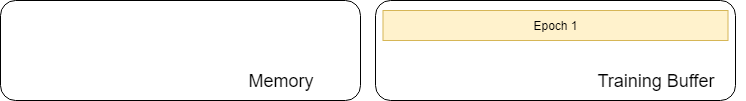
\includegraphics[width=\textwidth]{figures/CatastrophicForgettingA}
			\caption{First training. Since no training has occurred beforehand, the entire training buffer is used.}
	\end{subfigure}
	\begin{subfigure}{\linewidth}
		\centering
		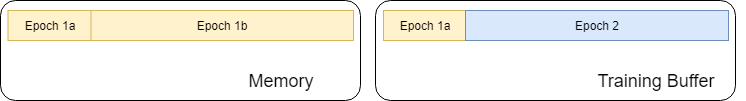
\includegraphics[width=\textwidth]{figures/CatastrophicForgettingB}
		\caption{Second training. Some of the first training epoch is kept, but most of it is replaced by new data from epoch 2.}
	\end{subfigure}
	\begin{subfigure}{\linewidth}
	\centering
	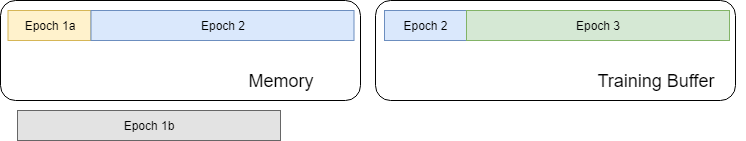
\includegraphics[width=\textwidth]{figures/CatastrophicForgettingC}
	\caption{Third training. All data from epoch 1 is no longer kept, and only data from epoch 2 is in the training buffer. A portion of epoch 1 is no longer in the memory of the MLP.}
	\end{subfigure}%
	\caption{A visual representation of how catastrophic forgetting occurs. \textbf{\textit[Use arrows to show idea more clearly.]}}
	
	\end{figure}
	\par One way to deal with this is to use a recursive training method, which updates the network based on batches of samples each time but uses these samples to update an internal state. The recursive implementation LM, as described by Ngia and Sjoberg \cite{placeholderCitation}, is used in this thesis. In this process, there is a forgetting factor $\alpha$ built in that allows for the network to forget past inputs in a more explicit manner than the standard batch-update method. In the following equations, $\varepsilon(h_t) = \sqrt{J(h_t)}$, $P_t$ can be considered the covariance matrix of the weights, $\Omega^T(h_t)$ is a modified gradient for y, allowing for a normalization factor $\rho$ to be added in one weight at a time. The second row of $\Omega^T(h_t)$ is 0 for all indices where $i\ mod\ (nWeights+1) \neq t$, and 1 where $i\ mod\ (nWeights+1) = t$. $\alpha$ is the rate of forgetting. 
	\begin{align}\label{bg:RLM_ref}
		\Omega^T(h_t) &= \begin{bmatrix}
			&& \nabla_y^T(h_t) && \\ 0 & ... & 1 & ... & 0
		\end{bmatrix} \\
		\Lambda_{T}^{-1} &= \begin{bmatrix}
			1&0\\0&\rho
		\end{bmatrix} \\
		S(h_t) &= \alpha_t\Lambda_t + \Omega^T(w_t)P_{t-1}\Omega(w_t) \\
		P_t &= \frac{1}{\alpha_t}[P_{t-1}-P_{t-1}\Omega(h_t)S^{-1}(h_t)\Omega^T(h_t)P_{t-1}]\\
		h_{t+1} &= h_t + P_t \nabla_y(h_t)\varepsilon(h_t) 
	\end{align}
	\par The update process is split into three substeps, each substep updating a a related aspect of the internal or external state of the NN. The first step computes an intermediate state $S(h_t)$, which reduces the necessary matrix inversion to a $2\times2$ matrix. The second step updates the covariance matrix, and finally the third step updates the weights. 
	\par A different approach for dealing with catastrophic forgetting is to use ensemble training methods \cite{placeholderCitation}. Ensemble methods use a collection of learners to produce improved results over any individual learner by itself. In general, ensemble methods use a set of weaker algorithms that are combined with or without some sort of weighting to produce a unified result \textbf{\textit{[look into visualization]}}. In classification problems, a weighted majority voting is often used while in regression problems a weighted median or mean can be employed. Frequently, a CART is used as the base algorithm due to its simple implementation and reasonable performance. However, any algorithm can be selected. Once a base algorithm is chosen, the difference between ensemble implementations is how the ensemble is created and used. For instance, in Adaboost \cite{placeholderCitation} a series of base learners is trained, where each successive base learner is trained in a way that more heavily weights points that the previously trained learners have trouble with. This differs from bagging \cite{placeholderCitation}, a different algorithm where each base learner is trained with a different subset of the total training data. These examples are provided simply to show how ensemble learning methods can differ.
	\par The method most relevant to addressing the problem of catastrophic forgetting is Learn++.NSE \cite{placeholderCitation}. For each window of samples, Learn++.NSE creates a new learner that is trained on the window. The samples in the training window are weighted by how much trouble the pre-existing learners had in predicting the value, ensuring that the new learner is better at recognizing these samples. It then weights the new learner and existing learners based on how well they work on the training data, using a metric such as MSE. In doing this, existing learners contribute to the resulting prediction based on how well they work on the most recent window of data. 
		\begin{algorithm}[ht!]
		\caption{Learn.NSE++ Pseudoalgorithm \textbf{\textit{[carry line breaks over moving things]}}}
		\label{bg:nseSection}
		\begin{algorithmic}[1]
			\Procedure{Learn.NSE++}{}
			\State $t=1,\ numActiveClassifiers = 0$ 
			\State $m^t$ is the data window size at epoch t.
			\While{Running}
			\If{$t = 1$} 
			\For{$i=1 \to numActiveClassifiers$}
			\State $D(i) = w(i) = 1/m^1$
			\EndFor
			\Else
			\State Apply data window to current ensemble. 
			\State $E^t = \sum^{m^t}(1/m^t) * squaredError($current learner, current data$)$
			\State At this point, $E^t$ should be a vector with size $m^t$.
			\For{$i = 1,i<numActiveClassifiers, i++$}
			\State Update learner weights: $w_i = 1/m^t * \sum squaredError($current learner, current data$)$
			\EndFor
			\State Normalize learner weights: $D = w \odot (1/\sum w)$
			\EndIf
			\If{ $numActiveClassifiers = numClassifiers$}
			\State Remove oldest classifier.
			\Else
			 $numActiveClassifiers = numActiveClassifiers + 1$
			\EndIf
			\State Train new Learner on new data window.
			\State Evaluate all existing classifiers with new data.
			\For{$i=1 \to numClassifiers$}
			\State $\epsilon_i^t = \sum D(i) * squaredError($ current learner, current data$)$
			\State $\beta_i^t = \epsilon_i^t/(1-\epsilon_k^t) $
			\State Compute average of normalized error for $h_i$: $\omega_i^t = 1/(1+exp(-a(t-i-b)))$
			\State $\omega_i^t = \omega_i^t / \sum_{j=0}^{t-i} \omega_i^{t-j}$
			\State $\hat{\beta_i^t} = \sum_{j=0}^{t-i} \omega_k^{t-j} \beta_i^{t-j}$
			\If{$t>numClassifiers$} 
			\State Calculate classifier voting weights $W_i^t = log(1/\hat{\beta_i^t})$
			\EndIf
			\EndFor
			\State Training Done.
			\While{Filling training buffer}
			\State get Hypothesis $H(x) =\sum_{i=0}^{numClassifiers} W_i^t * h_i(x) $
			\EndWhile
			\State Buffer full, $t += 1$.
			\EndWhile
			\EndProcedure
		\end{algorithmic}
	\end{algorithm}
	\par In the standard implementation of Learn++.NSE, a classification problem is targeted, and it is supposed that an infinite number of learners can be created. The adjustment from classification to regression requires the algorithm to use MSE instead of cross-entropy as an error function, and a method for limiting the number of learners is required as well. Due to time constraints, a simple pruning process of choosing a maximum number of learners and replacing the oldest learner was chosen. More complex pruning methods have been explored in \cite{placeholderCitation}.
	\clearpage
	\subsection {GANS, and evaluating the utility of them \textit{[retitle]}}
	\par One of the major goals of this extension to the previous work is to evaluate whether the concept of Generative Adversarial Networks (GANs) \cite{placeholderCitation} was applicable to the project. Like the cognitive engine in its current state, GANs are composed of two neural networks providing complementary data. In this section, GANS will be described in more detail, as well as their applicability to the CE.  
	\par The primary purpose of a GAN is to implicitly model some probabilistic data distribution. This is usually done in the case where data is either too complex to model effectively or completely unknown. Prior work has focused primarily on image-based data. Common datasets to be modeled for testing include MNIST (hand written digits), CIFAR-10 (natural images) and the Toronto Face Dataset (TFD) \cite{gan_overview}. These distributions happen to be all image-based, but there is no explicit need for the data distribution to be an image. Images just happen to be an extremely complicated representation space with many nonlinear patterns, making it a good data type for practice.
	\par A GAN is composed of two separate learners: a Generator($\mathcal{G}$) and a Discriminator($\mathcal{D}$). $\mathcal{G}$ and $\mathcal{D}$ are configured to be in competition,where $\mathcal{D}$ is attempting to distinguish between points that are generated by $\mathcal{G}$ and points that are sampled from the true distribution. $\mathcal{D}$ returns a 0 if it thinks the datapoint is not from the true distribution, and a 1 if it thinks the datapoint is. $\mathcal{G}$ is attempting to fool $\mathcal{D}$ into confusing its generated datapoints with the data from the true distribution. Its best case scenario is when $\mathcal{D}$ is only correct around 50\% of the time, as this makes $\mathcal{D}$'s prediction as good as randomly guessing which distribution the sample is from.
	\par In a more formal sense, $\mathcal{D}$ can be considered as dealing with a standard classification problem, attempting to classify whether or not a sample it is given is from the real distribution or the artificial one. $\mathcal{G}$ can be considered as dealing with a regression problem, trying to map a random uniform input $U(0,1)$ to the true distribution. 
	\par Figure \ref{bg:fig_ganDiagram} shows an overview of the GAN architecture. The task of $\mathcal{G}$, which is modeling a probability distribution, is more difficult than the task of the discriminator, $\mathcal{D}$, classification of incoming data. As such, when the discriminator ceases to improve, it is often frozen and only $\mathcal{G}$ gets updated. 
	\par The training of GANs is based on a value function $V(\mathcal{G},\mathcal{D})$, which is dependent on both the generator and the discriminator. Training the GAN accomplishes the following: 
	\[ \max_\mathcal{D}\min_\mathcal{G} V(\mathcal{G},\mathcal{D}) \], where:
	\begin{align}
		V(\mathcal{G},\mathcal{D}) &= E\{p_{real}\}log(\mathcal{D}(x)) + E\{p_{generated}\} log(1-\mathcal{D}(x)).
	\end{align}
	\par The competing nature of $\mathcal{G}$ and $\mathcal{D}$ is shown by the fact that one is trying to maximize the value function while the other is trying to minimize it. The first part of $V(\mathcal{G},\mathcal{D})$ represents the log-probability that the discriminator successfully classifies real datapoints as real. The second part represents the log-probability that the discriminator successfully classifies generated datapoints. $\mathcal{D}$ is thus trained by ascending the gradient of $V(\mathcal{G},\mathcal{D})$, and $\mathcal{G}$ is trained by descending a modified version of the gradient. Since $\mathcal{G}$ is only able to affect the probability of $\mathcal{D}$ providing a false positive, it only attempts to minimize this part of $V(\mathcal{G},\mathcal{D})$. Consequently, this becomes:
	\begin{align}
		\min_\mathcal{G} E\{p_{generated}\} log(1-\mathcal{D}(x)).
	\end{align}
	\par In order to use a non-saturating criterion, the minimization is rearranged to be a maximization:
	\begin{align}
		\max_\mathcal{G} E\{p_{generated}\} log(\mathcal{D}(x)). \label{eq:bg_nonsatG} 
	\end{align}
	\textit{\textbf{[REFRAME X TO BE G(z) IN THIS]}}
	\par Beyond the value function, standard gradient-based backpropagation methods are used for updating the networks. Both networks are trained in tandem: a batch of real samples is collected, a batch of generated samples are created, and then the results of feeding these samples through $\mathcal{D}$ are used to update both $\mathcal{D}$ and $\mathcal{G}$.  
	\begin{figure}
		\centering
		\caption{A flow diagram describing how GANs are structured.}
		\label{fig:GanFlowDiagram}
		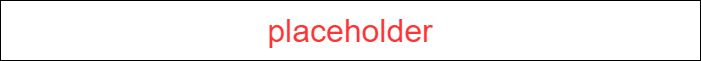
\includegraphics[scale=0.5]{figures/Placeholder.png}
	\end{figure}
	\par While GANs are a versatile method for modeling a data distribution, the training process is far from robust. The first issue is that there is no guarantee that the pair of models will converge. Due to the adversarial nature of the network, the convergence of a GAN depends on both models converging with competing objectives. The standard GAN procedure does not have any guarantees that this will happen. Another issue is mode collapse, when $\mathcal{G}$ starts to produce very similar samples for different inputs. This may result in good values for $V(\mathcal{G},\mathcal{D})$, but will only model a specific subset of the real data distribution. A final issue is that the loss value of $\mathcal{D}$ can quickly converge to zero, making there no reliable way to update $\mathcal{G}$. This is called the vanishing gradient problem \cite{placeholderCitation}, and is not specific to GANs. 
	\par In practice, there are a couple of approaches that are used to reduce the impact of these issues. One method is to normalize the inputs of each layer by subtracting the input mean and dividing by the input standard deviation \cite{placeholderCitation}. This ensures that inputs of vastly different magnitudes can be represented in a more similar manner. Doing this introduces a "standard deviation" parameter and a "mean" parameter for each node, allowing for the training process to use "denormalized" nodes if it is optimal without reducing the overall stability. This most directly affects the vanishing gradient problem, but also has positive effects on convergence rate as well.
	\par An approach used to deal with mode collapse is mini-batch discrimination \cite{placeholderCitation}, which adds an input to the discriminator that encodes the distance between a sample in a mini-batch and the other samples. This makes the discriminator able to tell if the generator is producing the same outputs. Another approach, called feature matching \cite{placeholderCitation} which alters the goal of $\mathcal{G}$ in order to try to match an intermediate activation of $\mathcal{D}$ from real samples with its generated samples. The additional information makes it more able to represent complex representations. Heuristic averaging \cite{placeholderCitation}, which penalizes network parameters if they stray from a running average of previous values, is a useful approach to aid in making the GAN converge. 
	\par Beyond the heuristic approaches, there have been a few attempts at alternative, more robust formulations of GANs. The most prominent approach is the WGAN \cite{bg:wganPaper}. This modifies the cost function of the GAN to use Wasserstein distance, instead of cross-entropy. The details of Wasserstein distance, also known as Earth-Mover distance, are irrelevant to this thesis, and so will be left for viewer investigation. However, the intuition of Wasserstein distance is that:  
	\begin{itemize}
		\item $P_x$ and $P_y$ are similar to piles of earth. 
		\item $\gamma(x,y)$ is the amount of "mass" that needs to be moved to make $P_x$ into $P_y$.
		\item Wasserstein distance is the "cost" of the optimal transport plan of $\gamma$.
	\end{itemize}
	Other interesting alternate GANs are DCGAN \cite{placeholderCitation} and ALI\cite{placeholderCitation}.
	\par On a surface level, the RLNN has some similarities to the GAN. As with a GAN, the RLNN uses two neural networks working in combination to produce different types of results. However, many of the similarities end here. The performance of the explore and exploit networks are not particularly related, as the performance of one does not indicate the performance of the other. Furthermore, neither the explore network nor the exploit network were developed as a classification problem. In order to make these networks fit the GAN structure, there would need to be a restructuring of the RLNN architecture.
	\par Another potential way to use the GAN is in replacement of the explore or exploit network. The explore network is the model that fits into the standard GAN formation. Indeed, it could be considered to be attempting a similar problem as $\mathcal{G}$. While there would be benefits of replacing the explore network with a GAN, limitations of the experiment setup prevent doing so. The amount of samples required to properly train a GAN would likely be prohibitive, considering how difficult it is to schedule time to conduct experiments on the space-based platform. As a result of this, the conclusion is that GANs are not directly applicable to the CE.
	
	\section{Summary}
	\par \textbf{\textit{[write actual summary]}}
%\end{document}